%
%  thesis.tex  2014-01-15  Mark Senn  http://engineering.purdue.edu/~mark
%
%  This is the thesis ``root file''.
%
%  To print the final copy of your thesis put a '%'
%  in front of the \includeonly command and type
%  (from page 71 of _LaTeX User's Guide and Reference Manual_, 2nd edition):
%      latex thesis
%      bibtex thesis
%      latex thesis
%      latex thesis
%
%  In "Reference:" listings below:
%      KEY  MEANING
%      TM   ``A Manual for the Preparation of Graduate Theses'',
%             seventh revised edition, The Graduate School, 2006.
%             http://www2.itap.purdue.edu/gradschool//Publications/graduate-thesis-manual.pdf
%      PU   ``A Manual for the Preparation of Graduate Theses'',
%           The Graduate School, Purdue University, 1996.
%           http://www2.itap.purdue.edu/gradschool//Publications/graduate-thesis-manual.pdf
%
%  Search for "CHANGE" below and change things as necessary.
%  I recommend putting "%%" before any existing lines that
%  need to be changed and adding your new line(s) immediately
%  below the existing lines.
%

% See http://www.ecn.purdue.edu/~mark/puthesis/#Options
% for documentclass options.
% CHANGE NEXT LINE?
\documentclass[ece,dissertation]{puthesis}

% Define "align" environment used in demo-mathematics.tex.
% CHANGE NEXT LINE?
\usepackage{amsmath}
\usepackage{color}
% Define "multicols" environment environment used in demo-multicols.tex.
% CHANGE NEXT LINE?
\usepackage{multicol}

% Define "subfigure" environment used in "demo-figure.tex".
% CHANGE NEXT LINE?
\usepackage{subfigure}
\usepackage{packages/algorithm}
\usepackage{packages/algorithmic}

% Title of thesis (used on cover and in abstract). The title shown must be the full, official title of the thesis.
% Superscripts and subscripts are not permitted in the title. Reference: TM 26.
% Use \title{Put Title Here} for a one-line title. Use \\ to separate lines.
% Put % at the end of the last line to avoid getting an extra space in the abstract.
% There are two forms of title: one line or more than one line.
% There are examples of both below.
% Only use one \title.
% CHANGE NEXT FOUR LINES.
% \title{An Example Thesis Done with LaTeX}
\title{%
  Secure data aggregation scheme\\
  for sensor networks%
}

% First author name with first name first is used for cover. Second author name with last name first is used for abstract.
% Your full name as it appears in the University records appears on the cover. Reference: TM 26, 29.
% There are two forms of author, with and without initials.
% There are examples of both below.
% Only use one \author line.
% CHANGE NEXT TWO LINES.
%\author{Mark Senn}{Senn, Mark}
%\author{Mark D. Senn}{Senn, Mark D.}
\author{Kavit Shah}{Shah, Kavit}

% First is long title of degree (used on cover).
% Second is abbreviation for degree (used in abstract).
% Third is the month the degree was (will be) awarded (used on cover
% and abstract).
% Last is the year the degree was (wlll be) awarded (used on cover
% and abstract).
% The degree title for all doctoral candidates is ``Doctor of Philosophy.''
% The precise degree names for master's candidates appear in the list of
% ``Degrees Offered'' in the Graduate School bulletin.
% The date is the month and year that the degree is actually awarded.
% (If you have registered for ``degree only,'' revise the thesis title
% page to reflect the new date on which the degree is to be awarded.)
% Reference: TM 26--27, 30.
% CHANGE NEXT LINE?
%\pudegree{Doctor of Philosophy}{Ph.D.}{May}{2007}
\pudegree{Master of Science in Electrical and Electronics Engineering}{Master}{December}{2014}

% Major professor (used in abstract).
% Use, for example:
%     \majorprof{John Q. Professor}
%     \majorprofs{John Q. Professor and Thomas R. Jones}
%     \majorprofs{John Q. Professor, Thomas R. Jones, and David S. Smith}
% depending on the number of major professors you have.
% CHANGE NEXT LINE.
\majorprof{Dr. Brian King}

% Campus (used only on cover)
% Use one of the following:
%     Fort Wayne
%     Hammond
%     Indianapolis
%     West Lafayette
%     Westville
% Reference: TM 27.
% CHANGE NEXT LINE?
\campus{Indianapolis}

% My command definitions not specific to my thesis.
% CHANGE NEXT LINE?
%
%  mydefs.tex  2007-03-19  Mark Senn  http://www.ecn.purdue.edu/~mark
%
%  Command definitions that can be used in all documents that have
%      %
%  mydefs.tex  2007-03-19  Mark Senn  http://www.ecn.purdue.edu/~mark
%
%  Command definitions that can be used in all documents that have
%      %
%  mydefs.tex  2007-03-19  Mark Senn  http://www.ecn.purdue.edu/~mark
%
%  Command definitions that can be used in all documents that have
%      \input{mydefs}
%

% CHANGE NEXT 3 LINES?
% Define \be and \ee to start and end the equation environment.
\newcommand{\be}{\begin{equation}}
\newcommand{\ee}{\end{equation}}

\newcommand{\tree}{$\mathcal{T}$}
\newcommand{\treeRoot}{$\mathcal{R}$}
\newcommand{\querier}{$\mathcal{Q}$}
\newcommand{\children}{$children$}
\newcommand{\parent}{$\mathcal{P}$}
\newcommand{\at}{$AggregationTree$}
\newcommand{\aggregator}{$A_{N}$}

\newcommand{\node}{$\mathcal{N}$}
\newcommand{\child}{$\mathcal{C}$}
\newcommand{\vertex}{$\mathcal{V}$}
\newcommand{\complainer}{$\mathcal{C}$}
\newcommand{\cheater}{$CHEATER$}
\newcommand{\lc}{$leftChild$}
\newcommand{\rc}{$rightChild$}

\newcommand{\cert}{$cert$}
\newcommand{\sign}{$SIGN$}
\newcommand{\msg}{$msg$}
\newcommand{\forest}{$forest$}
\newcommand{\nextTree}{$nextTree$}
\newcommand{\temp}{$temp$}
\newcommand{\height}{$height$}


% CHANGE NEXT 12 LINES?
% Define \Repeat so, for example,
%     \Repeat{whatever}{10}
% is the same as typing whatever 10 times.
\newcount{\myi}
\newcommand{\Repeat}[2]{%
    \myi=0
    \loop
        \ifnum\myi<#2
        #1
        \advance\myi by 1
    \repeat
}

% CHANGE NEXT 3 LINES?
% Make "\Sum ab" or "\Sum{a}{b}" do "\sum_{a}^{b}".
% This can only be used when in math mode.
\newcommand\Sum[2]{\sum_{#1}^{#2}}

% CHANGE NEXT 4 LINES?
% Make "\xn" do "$x_n$".
% Because this definition contains the "$" to go into math mode
% this definition must be used when not in math mode.
\newcommand{\xn}{$x_n$}

% CHANGE NEXT 5 LINES?
% Since \xn is already defined we must use \renewcommand to redefine it.
% Normally you would not have the above definition for \xn in this file
% if you were just going to override it later.
% The \ensuremath goes into math mode if not already in math mode.
\renewcommand{\xn}{\ensuremath{x_n}}


%

% CHANGE NEXT 3 LINES?
% Define \be and \ee to start and end the equation environment.
\newcommand{\be}{\begin{equation}}
\newcommand{\ee}{\end{equation}}

\newcommand{\tree}{$\mathcal{T}$}
\newcommand{\treeRoot}{$\mathcal{R}$}
\newcommand{\querier}{$\mathcal{Q}$}
\newcommand{\children}{$children$}
\newcommand{\parent}{$\mathcal{P}$}
\newcommand{\at}{$AggregationTree$}
\newcommand{\aggregator}{$A_{N}$}

\newcommand{\node}{$\mathcal{N}$}
\newcommand{\child}{$\mathcal{C}$}
\newcommand{\vertex}{$\mathcal{V}$}
\newcommand{\complainer}{$\mathcal{C}$}
\newcommand{\cheater}{$CHEATER$}
\newcommand{\lc}{$leftChild$}
\newcommand{\rc}{$rightChild$}

\newcommand{\cert}{$cert$}
\newcommand{\sign}{$SIGN$}
\newcommand{\msg}{$msg$}
\newcommand{\forest}{$forest$}
\newcommand{\nextTree}{$nextTree$}
\newcommand{\temp}{$temp$}
\newcommand{\height}{$height$}


% CHANGE NEXT 12 LINES?
% Define \Repeat so, for example,
%     \Repeat{whatever}{10}
% is the same as typing whatever 10 times.
\newcount{\myi}
\newcommand{\Repeat}[2]{%
    \myi=0
    \loop
        \ifnum\myi<#2
        #1
        \advance\myi by 1
    \repeat
}

% CHANGE NEXT 3 LINES?
% Make "\Sum ab" or "\Sum{a}{b}" do "\sum_{a}^{b}".
% This can only be used when in math mode.
\newcommand\Sum[2]{\sum_{#1}^{#2}}

% CHANGE NEXT 4 LINES?
% Make "\xn" do "$x_n$".
% Because this definition contains the "$" to go into math mode
% this definition must be used when not in math mode.
\newcommand{\xn}{$x_n$}

% CHANGE NEXT 5 LINES?
% Since \xn is already defined we must use \renewcommand to redefine it.
% Normally you would not have the above definition for \xn in this file
% if you were just going to override it later.
% The \ensuremath goes into math mode if not already in math mode.
\renewcommand{\xn}{\ensuremath{x_n}}


%

% CHANGE NEXT 3 LINES?
% Define \be and \ee to start and end the equation environment.
\newcommand{\be}{\begin{equation}}
\newcommand{\ee}{\end{equation}}

\newcommand{\tree}{$\mathcal{T}$}
\newcommand{\treeRoot}{$\mathcal{R}$}
\newcommand{\querier}{$\mathcal{Q}$}
\newcommand{\children}{$children$}
\newcommand{\parent}{$\mathcal{P}$}
\newcommand{\at}{$AggregationTree$}
\newcommand{\aggregator}{$A_{N}$}

\newcommand{\node}{$\mathcal{N}$}
\newcommand{\child}{$\mathcal{C}$}
\newcommand{\vertex}{$\mathcal{V}$}
\newcommand{\complainer}{$\mathcal{C}$}
\newcommand{\cheater}{$CHEATER$}
\newcommand{\lc}{$leftChild$}
\newcommand{\rc}{$rightChild$}

\newcommand{\cert}{$cert$}
\newcommand{\sign}{$SIGN$}
\newcommand{\msg}{$msg$}
\newcommand{\forest}{$forest$}
\newcommand{\nextTree}{$nextTree$}
\newcommand{\temp}{$temp$}
\newcommand{\height}{$height$}


% CHANGE NEXT 12 LINES?
% Define \Repeat so, for example,
%     \Repeat{whatever}{10}
% is the same as typing whatever 10 times.
\newcount{\myi}
\newcommand{\Repeat}[2]{%
    \myi=0
    \loop
        \ifnum\myi<#2
        #1
        \advance\myi by 1
    \repeat
}

% CHANGE NEXT 3 LINES?
% Make "\Sum ab" or "\Sum{a}{b}" do "\sum_{a}^{b}".
% This can only be used when in math mode.
\newcommand\Sum[2]{\sum_{#1}^{#2}}

% CHANGE NEXT 4 LINES?
% Make "\xn" do "$x_n$".
% Because this definition contains the "$" to go into math mode
% this definition must be used when not in math mode.
\newcommand{\xn}{$x_n$}

% CHANGE NEXT 5 LINES?
% Since \xn is already defined we must use \renewcommand to redefine it.
% Normally you would not have the above definition for \xn in this file
% if you were just going to override it later.
% The \ensuremath goes into math mode if not already in math mode.
\renewcommand{\xn}{\ensuremath{x_n}}




% My command definitions specific to my thesis.

% CHANGE NEXT LINE TWO LINES?
% Set things up so \margins will show where the margins on the page are.
\newcommand{\margins}{\Repeat{Show where the margins for the page are.}{4}}

% CHANGE NEXT TWO LINES?
% Let typing "\en" be exactly the same as typing "\ensuremath". 
\let\en=\ensuremath

% CHANGE NEXT FIVE LINES?
% Define a \ve command with two arguments, so if it called with
%     \ve an
% it will expand to
%     {\en{a_1},~\en{a_2},\ \ldots,~\en{a_{n}}}
\newcommand{\ve}[2]{\en{#1_1},~\en{#1_2},\ \ldots,~\en{#1_{#2}}}


% To LaTeX only some parts of your thesis put the
% names of the parts to include here.  For example,
% \includeonly{front} would only process front.tex.
% \includeonly{front,introduction} would only process
% front.tex and introduction.tex.
% To print the final copy of your thesis put a '%'
% in front of the \includeonly command and run LaTeX
% three times to make sure that all cross-references
% are correct.  Then run BibTeX once and LaTeX twice
% more.
% CHANGE NEXT LINE?
%\includeonly{front,introduction}
\newcommand{\node}{\textsf{node}}

\begin{document}

	% Start a new volume for your thesis.  All theses must have at least one
	% volume.  If your thesis is too long to fit in one binder put another
	% "\volume" between chapters below.
\volume

% Front matter (dedication, etc.).

%
%  revised  front.tex  2011-09-02  Mark Senn  http://engineering.purdue.edu/~mark
%  created  front.tex  2003-06-02  Mark Senn  http://engineering.purdue.edu/~mark
%
%  This is ``front matter'' for the thesis.
%
%  Regarding ``References'' below:
%      KEY    MEANING
%      PU     ``A Manual for the Preparation of Graduate Theses'',
%             The Graduate School, Purdue University, 1996.
%      TCMOS  The Chicago Manual of Style, Edition 14.
%      WNNCD  Webster's Ninth New Collegiate Dictionary.
%
%  Lines marked with "%%" may need to be changed.
%

  % Dedication page is optional.
  % A name and often a message in tribute to a person or cause.
  % References: PU 15, WNNCD 332.
% \begin{dedication}
%   This is the dedication.
% \end{dedication}

  % Acknowledgements page is optional but most theses include
  % a brief statement of apreciation or recognition of special
  % assistance.
  % Reference: PU 16.
\begin{acknowledgments}
  I would like to express my special appreciation and thanks to my advisor Dr.Brian King who has been my teacher, guide and mentor during the entire thesis and Master's program.
  I am grateful to him for being a great role model for researcher, teacher and a leader in my life.
  I would like to thank him for encouraging my research and for allowing me to grow as a researcher.
  % Your advice on both research as well as on my career have been priceless

  I would also like to thank the other members of my thesis committee: Paul Salama, Mohamed El-Sharkawy and Sangkook Lee for their assistance during the thesis.
  % I would like to thank them for their constructive feedback during the collaboration. 
  I want to thank them for letting my defense be an enjoyable moment, and for their brilliant comments and suggestions. 

  I would also like to thank the entire Academic staff of Electrical and Computer Engineering Department at Indiana University Purdue University - Indianapolis for begin so nice and helpful all the time. 

  Finally, I would like to thank my family for being patient and loving all the time.
  My family's financial and emotional support for me has been incredible.
  Their prayers for me was what sustained me thus far.    

\end{acknowledgments}

  % The preface is optional.
  % References: PU 16, TCMOS 1.49, WNNCD 927.
% \begin{preface}
%   This is the preface.
% \end{preface}

  % The Table of Contents is required.
  % The Table of Contents will be automatically created for you
  % using information you supply in
  %     \chapter
  %     \section
  %     \subsection
  %     \subsubsection
  % commands.
  % Reference: PU 16.
\tableofcontents

  % If your thesis has tables, a list of tables is required.
  % The List of Tables will be automatically created for you using
  % information you supply in
  %     \begin{table} ... \end{table}
  % environments.
  % Reference: PU 16.
\listoftables

  % If your thesis has figures, a list of figures is required.
  % The List of Figures will be automatically created for you using
  % information you supply in
  %     \begin{figure} ... \end{figure}
  % environments.
  % Reference: PU 16.
\listoffigures

  % List of Symbols is optional.
  % Reference: PU 17.
\begin{symbols}
  % $s$& Sensor node \cr
  $N$& Query nonce\cr
  $H$& Hash function\cr
  % $d$& Distance \cr
  % $D$& Data-item \cr
  % $X$& Random variable \cr
  % $\delta$& Fanout of a sensor node \cr
  % $f$& Function \cr
  % $v$& Vertex \cr
  % $A$& An attack \cr
  % $\alpha$& Resilient factor \cr
\end{symbols}

  % List of Abbreviations is optional.
  % Reference: PU 17.
\begin{abbreviations}
  ACK& Positive acknowledgment message\cr
  BER& Bit error rate\cr
  MAC& Message Authentication Code\cr
  NACK& Negative acknowledgment message\cr
  SHA& Secure hash algorithm\cr
  SIA& Secure information aggregation\cr
  SHIA& Secure hierarchical in-network aggregation\cr
\end{abbreviations}

  % Nomenclature is optional.
  % Reference: PU 17.
% \begin{nomenclature}
%   Alanine& 2-Aminopropanoic acid\cr
%   Valine& 2-Amino-3-methylbutanoic acid\cr
% \end{nomenclature}

  % Glossary is optional
  % Reference: PU 17.
% \begin{glossary}
%   chick& female, usually young\cr
%   dude& male, usually young\cr
% \end{glossary}

  % Abstract is required.
  % Note that the information for the first paragraph of the output
  % doesn't need to be input here...it is put in automatically from
  % information you supplied earlier using \title, \author, \degree,
  % and \majorprof.
  % Reference: PU 17.
\begin{abstract}
  % We show that 

  % We show that two distinguishing properties of sensor networks, i.e., the presence of a trusted base station, and the pre-knowledge of the fixed network topology, can yield security protocols that are both communication-efficient and highly general. 
  
  We propose a secure in-network data aggregation protocol with internal verification, to increase the lifetime of the sensor network by preserving bandwidth.
  For doing secure in-network distributed computations, we show an algorithm for securely computing the sum of sensor readings in the network.
  Our algorithm can be generalized to any random tree topology and can be applied to any combination of mathematical functions.
  In addition, we represent an efficient way of doing statistical analysis for the protocol.
  Furthermore, we propose a novel, distributed and interactive algorithm to trace down the adversary and remove it from the network.   
  Finally, we do bandwidth analysis of the protocol and give the proof for the efficiency of the protocol.

\end{abstract}


% Put chapter \include commands here.
% CHANGE \include{...} COMMANDS BELOW?
%
%  revised  introduction.tex  2011-09-02  Mark Senn  http://engineering.purdue.edu/~mark
%  created  introduction.tex  2002-06-03  Mark Senn  http://engineering.purdue.edu/~mark
%
%  This is the introduction chapter for a simple, example thesis.
%


\chapter{Introduction}

	% This is the introduction.
	% The first paragraph after a heading is not indented.
	TIPS:
		USE ACTIVE VOICE\\
		USE VERBS\\
		DON'T TURN VERBS INTO NOUNS

	COMMON MISTAKE:
		DATA ARE ; DATA IS PLURAL
		THAT/WHICH

	Advancements in compute, storage, networks and sensors technologies have led to many new promising applications. 

	% This is a sentence.
	% This is a sentence.
	% This is a sentence.
	% This is a sentence.
	% This is a sentence.
	\section{Sensor Networks}

		The sensor networks of the near future are envisioned
		to consist of hundreds to thousands of inexpensive
		wireless sensor nodes, each with some computational power
		and sensing capability, operating in an unattended mode.
		They are intended for a broad range of environmental sensing
		applications from vehicle tracking to habitat monitoring.
		Give an example and talk about energy, security constraints.

	\section{Internet Of Things}

		In the world of mass connectivity people need to get information all the time on an array of devices. Everything from your refrigerator to your thermostat is connected to wireless networks and joining the ``internet of things''. Write about bandwidth constraints.

	\section{Big Data}
		All the large internet companies process massive amounts of data also know as ``Big Data'' in real time applications.
		These include batch-oriented jobs such as data mining, building search indices, log collection, log analysis, real time stream processing, web search and advertisement selection on big data.
		To achieve high scalability, these applications distributes large input data set over many servers.
		Each server process its share of the data, and generates local intermediate.
		The set of intermediate results contained on all the servers is then aggregated to generate the final result.
		Often the intermediate data is large so it is divided across multiple servers which perform aggregation on a subset of the data to generate the final result. 
		If there are \emph{N} servers in the cluster, then using all \emph{N} servers to perform the aggregation provides the highest parallelism. Talk about compute constraints.
		\cite{Goossens:1994}
		
		Airplanes are also a great example of ``big data''. 
		In a new Boeing Co.747, almost every part of the plane is connected to the Internet, recording and sometimes sending continuous streams of data about its status.
		According to General Electric Co. in a single flight one of its jet engines generates half a tera bytes of data.
		This shows that we have too much of data and we are just getting started.

	\section{Data Aggregation}

		Data aggregation is an important technique used in many system architectures. 
		The key idea is to combine the data coming from different sources eliminating the data redundancy, minimizing the number of packet transmissions thus saving energy, bandwidth and memory usage.
		This technique allows us to focus more on data centric approaches for networking rather than address centric approaches.  \cite{krishnamachari2002impact}  

	\section{Cloud Computing}

	\section{Fog Computing}

		\subsubsection{}


\chapter{Related Work}

\section{Secure Aggreagation}

David Wagner in Resilient Aggregation in Sensor Networks describes various attacks on aggregation schemes and introduces stastical estimation theory to secure aggregation. It helps deciding secure aggregation function by defining function is resilient or not.

SIA: Secure Information Aggregation in Sensor Networks proposes secure aggragation scheme for single-aggregator model. It provides stastical security properties. 

In contrast, our work presents an approach for the more genral multi-hop aggregation model.

\chapter{Problem Statment and Assumptions}

\section{Assumptions}
1. Trusted Querier
2. Leaves can report only one value at a time.
3. pre-knowledge of network topology
\chapter{Secure Data Aggregation Scheme}

	The goal of this thesis is to examine secure data aggregation schemes for various distributed systems. 

	Many modern world system designs are distributed in nature. The system design includes small, individual components doing their tasks precisely and lots of these components synchronize with all other components to complete the bigger task.  


	Many applications of sensor network are inharenlty distributed in nature.
	For example, scientific data collection, building health monitoring , building safety monitoring systems are distributed systems.
	Write an example how data aggregation happes in one particular application.\cite{wagner2004resilient}

	The application design architecture for the internet of things is distributed as well. Write an example how data aggregation happens in one particular application.
	\cite{green1982analysis}


%
%
\section{Network topology}

%This is a sentence.
%This is a sentence.
Write about how all theses distributed systems can be classifieds into general tree structure.


\subsubsection{Subsubsection heading}

This is a sentence.
This is a sentence.

	
\chapter{Commitment Tree Generation}

\begin{theorem}
%\emph{(Lagrange's Theorem)}
\label{Commitment tree}
Binary commitment tree is optimal for terms of verification as it requires minimum number of off-path values.
\end{theorem}

\begin{proof}
Let us say 

$ \log _3( n ) = y $

$ 3^y = n $

$ \log_2( 3^y ) = \log_2( n ) $

$ y * \log_2( 3 ) = \log_2( n ) $

$ \log_3( n )*\log_2( 3 ) = \log_2( n ) $

$ \log_3( n ) = \frac{ {\log _2 ( n )} }{{\log _2 ( 3 )}} $

$ 2 * \log_3( n ) = [2 / \log_2( 3 ) ]* log_2( n ) = ( 1.2618 ) * log_2( n ) $

$ 2 * log_3( n ) > log_2( n ) $  

\end{proof}
\chapter{Verification of confirmations}

\section{Network Model}

We assume a multihop network with a set $ S = \{s1,...,s_{n}\} $ of $n$
sensor nodes. The network is organized in a tree topology, with the
base station as the root of the tree. The trusted querier resides
outside of the network \& has more computation, storage capacity 
then the sensor nodes in the network. The querier knows total number of sensor nodes $n$ and that all $n$ nodes are alive and reachable. The querier also knows the network topology. 
All the wireless comuunication is peer-to-peer and we do 
not consider local wireless broadcast. We also assume that the
querier has the capacity to do peer to peer communication with 
every sensor node in the network. We also assume that all the sensor nodes 
mapped to the vertices in the commitment tree who reported the authentication 
codes with NACK messages during the collection of confirmations step are 
honest. 

\subsection{Sensor Nodes}

	We assume that each sensor node has a unique identifier $s$ and
	shares a unique secret symmetric key $K_{s}$ with the querier. 
	We assume all the sensor nodes are capable of doing symmetric-
	key encryption and symmetric key decryption. They are also
	capable of computing collision-resistant cryptographic hash 
	function $H$. We also assume that if the sensor node has to send 
	multiple messages to its parent it can combine those messages 
	into single packet in a way that parent node can distinguish both 
	the messages.

\subsection{Commitment trees} % (fold)
\label{sub:Commitment trees}
		
	The aggregation tree is a physical network over which all the
	communication happens while the commitment tree is a logical
	network on top of aggregation tree. In the similar manner, 
	vertices in a commitment tree is a logical element in a graph 
	while a sensor node is a physical device. 

	The commitment trees have the following properties. 
	At most there will be $\lceil lg  n \rceil$ commitment trees in the forest for an aggregation tree with $n$ sensor nodes.
	The binary representation of the number of sensor nodes $n$ in the network indicates the number of commitment trees in the forest. It also indicates the height of all the commitment trees in the forest. 
	For instance, if there are $ 11_{10} = 1011_{2} $ sensor nodes in the aggregation tree then there will be three commitment trees in the forest. From those three commitment trees, one will be of height three, one will be of height one and one will be of height zero.
	At most there will be $n + ( n - 1 )$ vertices in the forest of commitment trees for an aggregation tree with $n$ sensor 
	nodes.

	\textit{It is also possible that only one sensor node $s$ in the aggregation tree, will be the root vertex of all the commitment trees in the forest.} 

	\textit{It is also poosible that all the internal vetices in the commitment tree are of different sensor nodes in the aggregation tree.}


% subsection Commitment trees (end)

\subsection{Collections of confirmations}
After each sensor node $s$ has successfully performed the 
verification step for its leaf vertex $u_{s}$, it sends an 
authentication code to its parent in the aggregation tree.
The authentication code for sensor node $s$ is MAC$_{K_{s}}(N||ACK)$
where ACK is an acknowledgemnet message, N is the query nounce and $K_{s}$ 
is the secret key that sensor node $s$ shares with the trusted querier. Once
an internal sensor node $s$ in the aggregation tree has received the
authentication codes from all of its descendants, it computes the XOR of its 
own authentication code with all the received authentication codes, and 
forwards the result to its parent. Finally, the querier will receive a 
single authentication code from the base station that consists of the XOR of 
all the authentication codes received in the network. 

\subsection{Verification of confirmations}
Since the querier knows the secret key $K_{s}$ for each sensor node $s$ in the aggregation tree and it also knows the topology of the commitment trees in the forest, it can simulate the commitment trees in the forest. The querier simulates the commitment trees in the forest by computing the following authentication codes\\

MAC$_{K_{1}}(N||ACK)\,\oplus\,$ 
MAC$_{K_{2}}(N||ACK)\,\oplus\,$
...
$\,\oplus\,$
MAC$_{K_{n}}(N||ACK)$ ; \\
MAC$_{K_{1}}(N||NACK)\,\oplus\,$ 
MAC$_{K_{2}}(N||NACK)\,\oplus\,$
...
$\,\oplus\,$
MAC$_{K_{n}}(N||NACK)$  \\


and creates two simulated commitment trees, one with the authentication codes of ACK messages and one with the authentication codes of NACK messages; where ACK is an acknowledgemnet message, NACK is a negative acknowledgemnet message \& N is the query nounce. Then the querier merges all the commitment trees in the forest simulated with the authentication codes of ACK messages, by taking XOR of the root of all the commitment trees in the forest and calculates a single root authentication code for the forest simulated with the authentication codes of ACK messages. The querier does the same procedure for the commitment trees' forest simulated with the authentication codes of NACK messages. The querier stores all the simulated commitment trees and root authentication codes in the memory. \\


The querier receives a signle root authentication code from the base station during the collection of confirmation messages step. The querier compares the received root authentication code with the relevant simulated authentication code of ACK messages. If those two codes match it means every vertices in the subtree rooted at that vertex sent the authentication codes with ACK message during collection of confirmation step. If those two codes do not match it means one or more vertices in the subtree rooted at that vertex sent the authentication codes with NACK message during collection of confirmation step. In the case where root authentication codes do not match, the querier proceeds futher to find out which vertex or vertices in the network sent the authentication codes with NACK message during collection of confirmation messages step.\\


To find out which vertex or vertices in the commitment tree reported the authentication codes with NACK message, the querier asks the base station to send the authentication codes of all the commitment trees' root in the forest. After receiving the authentication codes from the base station, the querier compares those authentication codes with the relevant simulated authentication codes of ACK messages. After this comparision, whose authentication codes do not match, the querier classifies those commitment trees as BAD TREES in the forest. \\


Then the querier compares the authentication codes of those BAD TREES with the relevant simulated authentication codes of NACK messages. If any of those authentication codes match it means all the vertices rooted in that subtree sent the authentication codes with NACK message during the collection of confirmation stpe. And the querier stops doing the quiers to the subtree rooted at that vertex. If those authentication codes do not match then the querier proceeds furhter to find the senosr node or nodes who reported the authentication codes with NACK message in BAD TREES.\\


\subsection{Algorithm for detecting vertex or vertices who reported authenctication codes with NACK messages }

For each BAD TREE in the forest the querier does the following :

\begin{enumerate}
 
   \item 
  The querier asks the relevant nodes in the aggregation tree to send the authentication codes of their children in the commitment trees.

  \item
  The querier compares the received authentication codes in step 1 with the authentication codes of the relavant vertices of the commitment trees simulated with the authentication codes of ACK messages. The querier classifies the subtree rooted at those vertices as BAD SUBTREES, whose authentication codes do not match.

  \item 
  The querier compares the received authentication codes in step 1 with the authentication codes of the relavant vertices of the commitment trees simulated with the authentication codes of NACK messages. If those codes match it means all the vertices rooted in that subtree reported NACK messages during collection of confirmation steps. And the querier stops doing the queries to that subtree. If those codes do not match then the querier goes to step 2. \\

  The querier follows this algorithm until it finds all the vertices who reported the authentication codes with NACK messages in the commitment trees during collection of confirmation step.

\end{enumerate}




\subsection{Analysis} % (fold)
\label{sub:analysis}

To simulate the commitment trees in the forest the querier has to do the following calculations. Suppose there are $n$ sensor nodes in the network, means there will be at most $\lceil lg n \rceil$ commitment trees in the forest. If there are $n^{'}$ leaves in each commitment tree in the forest then the height($h^{'}$) of each commitment tree will be $lg(n^{'})$ and the number of intermediate vertices ($i^{'}$) in the network will be ($ 2^{h^{'}} - 1 $). So, there will be total of  $ (n^{'} + i^{'}) $ * $\lceil lg  n \rceil $  vertices in the forest. As the querier needs to simulate two commitment trees one for ACK messages and one for NACK messages it has to do ( $ 2 * (n^{'} + i^{'}) * \lceil lg  n \rceil $ ) calculations.

As we know from the properties of commitment trees, at most there 
will be $n + ( n - 1 )$ vertices in the forest of commitment trees 
for an aggregation tree with $n$ sensor nodes. So, the querier has
to do $ 2 * ( n + ( n - 1 ) )$ calculations and it also need that much memory space to store those values.

With Dr.King with a single NACK message in a tree:

Maximum number of leaves in a single commitment tree is equal to $n$. 
So, we can upper bound it with $O(n)$. As there is a signle NACK 
message in the tree, during verification phase we know in which part 
that vertex is. 

So, we can identify the node in at most $\log{n}$ steps.
We need $2*\log{n}$ messages to identify that. The querir will have to 
ask $\log{n}$ times and some node from the aggregation time has to 
reply $\log{n}$ times. This is total number of messages is required but 
number of communication depends on the aggregation tree.

Worst case:
In the worst case, the querier has to ask values of all the vertices in 
the commitment tree. At max there will be $(2*n - 1)$ messages. Again, 
remember these are the number of messages, number of communications 
might be different.

Best case in terms of number of communications:
It needs minimum number of communications when one single node is
everywhere in the aggregation tree. In that case if the querier has to 
know the values of all the leaves vertices it has to ask $\log(n)$ 
questions and node has to reply to those messages. So, number of 
communication is equal to $2 *log(n)$.


% subsection analysis (end)

\begin{figure}[t]
	\centering
		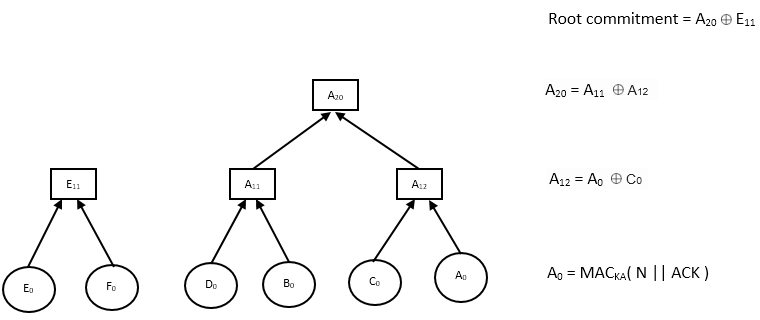
\includegraphics[width=0.8\textwidth]{ack.png}\\
		\caption{Simulated commitment tree with ACK messages}
	\label{fig:figure1}
\end{figure}

\begin{figure}[t]
	\centering
		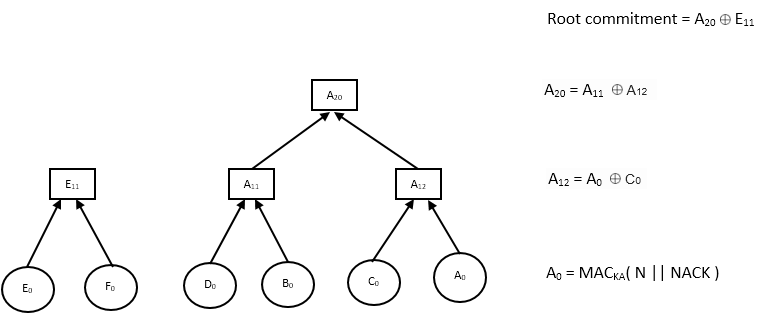
\includegraphics[width=0.8\textwidth]{nack.png}\\
		\caption[Simulated commitment tree with NACK messages]{Simulated commitment tree with NACK messages}
	\label{fig:figure1}
\end{figure}


\chapter{Cheating}

\section{Definition}
If an aggregator changes the sensor readings reported by its children to skew the final aggregated result is consider as cheating.

\section{Aim}
Aim of this section is to detect the cheater with given definition. 

\section{Assumptions}
We make an assumption that the cheater can not say NACK during verification phase. If a cheater is allowed to send NACK message then it can send NACK messages all the time and create a lot of traffic in the network which might create Denial of service attack. 

\section{What is not cheating ?}
	
	In figure 7.1, A is an aggregator if A is a cheater it can skew the final aggregation result irrespective of B's sensor reading. We do not consider this case as a cheating because A is adjusting its sensor reading, it's not changing the B's sensor reading. 
  
	For example, if maximum allowed value = 10\\
  
  case I: $B_{0}(2)$ = 5, $A_{0}(2)$ = 13, $A_{1}(2)$ = 18. In verification, A will be caught due to out of range off path value.\\

  case II: $B_{0}(2)$ = 5, $A_{0}(2)$ = 10, $A_{1}(2)$ = 15. $B_{0}^{'}(2)$ = 6, $A_{0}^{'}(2)$ = 9. that's not cheating.\\ 

	\begin{figure}[t]
		\centering
			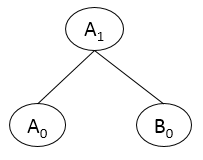
\includegraphics[width=0.2\textwidth]{commitment_tree_1.png}\\
			\caption{Possible commitment tree}
	\end{figure}

	Similar arguments can be done for figure 7.2 if A, C  both are cheaters. In that case A is adjusting C's sensor reading to skew the final aggregation result and C will not complain as it is a cheater. We do not consider that as cheating either.

\begin{figure}[t]
	\centering
		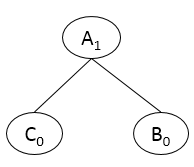
\includegraphics[width=0.2\textwidth]{commitment_tree_2.png}
		\caption{Possible commitment tree}
	\end{figure}

\section{Probabilistic bound on a cheater}
	
	To derive Probabilistic bound on a cheater using following example.

	In figure 7.3, all vertices in a commitment tree are unique. And, remember cheater can not say NACK during verification phase. 

	\begin{itemize}
		
		\item $A_{0}$ says NACK during verification phase it implies that atleast one of the following is \{I\}, \{B, I\}, \{B, M\} is a cheater.
		
		\item $A_{0}, B_{0}$ says NACK during verification phase it implies that atleast one of the following is \{I\}, \{M\}, \{C, D, O\} is a cheater.

		\item $A_{0}, B_{0}, C_{0}$ says NACK during verification phase it implies that atleast one of the following is \{J ,I\}, \{J, M\}, \{D, O\} is a cheater.

		\item $A_{0}, B_{0}, C_{0}, D_{0}$ says NACK during verification phase it implies that atleast one of the following is \{O\}, \{M\}, \{I, J\}, \{E, F, G, H, O\} is a cheater.

		\item $A_{0}, B_{0}, C_{0}, D_{0}, E_{0}$ says NACK during verification phase it implies that atleast one of the following is \{O, K\}, \{M, K\}, \{I, J, K\}, \{F, G, H, O\} is a cheater.

		\item $A_{0}, B_{0}, C_{0}, D_{0}, E_{0}, F_{0}$ says NACK during verification phase it implies that atleast one of the following is \{I, J, K\}, \{M, N\}, \{O, K\}, \{O, N\} is a cheater.

		\item $A_{0}, C_{0}$ says NACK during verification phase it implies that atleast one of the following is \{I\}, \{J\} is a cheater.

	\end{itemize}	

	\begin{figure}[t]
		\centering
			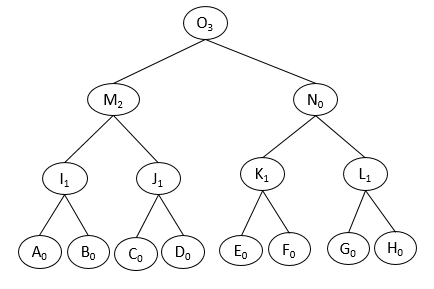
\includegraphics[width=0.7\textwidth]{commitment_tree_3.png}
			\caption{Possible commitment tree}
	\end{figure}

	Similar, kind of analysis can be done for figure 7.4 in which all the vertices in the commitment tree are different. 

	\begin{figure}[t]
		\centering
			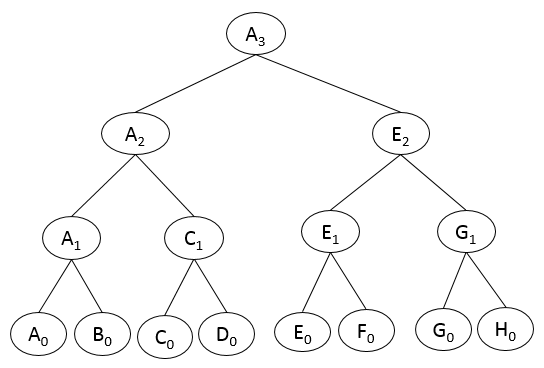
\includegraphics[width=0.7\textwidth]{commitment_tree_4.png}
			\caption{Possible commitment tree}
	\end{figure}

	From all above examples we can derive the following pattern as well,

	If d = depth of a tree,\\

	\begin{tabular}{| l | l |}
    \hline
    Depth of a cheater & Minimum number of NACK messages \\ \hline
    d - 1 & 1 \\ \hline
    d - 2 & 2 \\ \hline
    d - 3 & 4 \\ \hline
    d - 4 & 8 \\ \hline
  \end{tabular}


	\section{ Why do we need digital signatures ?}
	Digital signatures allow us to achieve authenticity of the message. 
	The labels and signatures have the following format:

	id = id

	label = $<count, value, commitment>$

	signature = $E_{Private_key}( H( N || label ) )$\\
	Where \textit{count} is the number of leaf vertices in the subtree rooted at this vertex; 
	\textit{value} is the SUM aggregate computed over all the leaves in the subtree; \textit{id} is the sum of all the leaves id in the subtree; \textit{signature} is a cryptographic scheme for demonstrating the authenticity of a message; \textit{N} is the query nonce. 
	
	There is one leaf vertex $u_{s}$ for each sensor node s, which we call the leaf vertex of s. The label of $u_{s}$ consists of count = 1, value = $a_{s}$ where $a_{s}$ is the data value of s, and signature is the node's unique ID.

	Internal vertices represent aggregattion operations, and have labels that are defined based on their children. Write up examples after talking to Dr.King : Do you have to aggregate ID's as well ?

	\section{ Why digital signatures are not sufficient to detect a cheater ? or Why do we need public key infrastructure to detect a cheater ?}
	Digital signatures allow us to achieve authenticity of the message but do not provide any mechanism to achieve integrity of the message. To achieve integrity we need public key infrastructure. 

	For example, in figure 7.3 one set of possible lables could be the following:

	$id_{A} = 1; A_{0} = <1, 5, H(N||1||5)>; Sig A_{0} = E_{K_{A}}(H(N||A_{0})); $

	$id_{B} = 2; B_{0} = <1, 6, H(N||1||5)>; Sig B_{0} = E_{K_{B}}(H(N||B_{0})); $

	$id_{I} = 3; I_{1} = <2, 11, H(N||2||11||A_{0}||B_{0})>; Sig I_{1} = E_{K_{I}}(H(N||I_{1})); $

	$id_{J} = 4; J_{1} = <2, 15, H(N||2||15||C_{0}||D_{0})>; Sig J_{1} = E_{K_{J}}(H(N||J_{1})); $

	$id_{M} = 5; M_{2} = <4, 26, H(N||4||26||I_{1}||J_{1})>; Sig M_{2} = E_{K_{M}}(H(N||M_{2})); $

	Above labels and signatures are the case where no one is cheating in the network. If A, B say NACK message during the verification phase it means either M or I is a cheater. To preceisely find who is cheater we have following problems:

	\begin{itemize}
		\item M can say it received ($I_{1}^{'}, Sig I_{1}$) eventhough it received ($I_{1}, Sig I_{1}$) from I.
		\item M can not verify that it received ($I_{1}^{'}, Sig I_{1}$) instead of ($I_{1}, Sig I_{1}$) from I.
	\end{itemize}
	Because of this we can not not detect cheater between I, M. The fundamental problem is that signatures can be verified only by the base station and not by any of the intermediate nodes. We want the ability in which an intermediate node can verify the signatures from its children. And that is why we need public key infrastructure.


%\chapter{performance-analysis}

\section{ A Notations }
	We are enhancing the analysis done in \cite{alzaid2008secure}.
	We consider the case in which intermediate nodes are sensors as well as aggregators, which makes network homogeneous. 
	According to us these scenario is more practical as it allows any node to be an intermediate node  according to the current state of the network and also allows dynamism in the network. We keep the same notations used in \cite{alzaid2008secure} to be consistent.

\section {B Number of transmitted bits}
	First, we start analyzing the case in which no aggregation and no security are used.
	Suppose all nodes in the network sends raw or encrypted data($x$ bits), sensor node ID data($y$ bits) and overhead data($oh$ bits) towards its parents which are $x+y+oh$bits long.
	Total number of bits traveled within the network is approximately, 
	\begin{equation}
				
	\end{equation}
	Special thing about your analysis is that you consider the case where aggregators are sensors as well. DO NOT FORGET TO INCLUDE IT.

\chapter{August}

Things discussed in meeting:
	
	Analyzed congestion and why is it sub linear ?
	
	In SHIA leaves verify their values with final results not with intermediate results. But in surveillance application data is compared with some base value in such network intermediate values are important. 

	Analyze the protocol with Digital signatures. How many signatures do we need ?

	Analyze properties of commitment tree.


\textbf{Definitions}

A \textbf{direct data injection attack} occurs when an attacker
modifies the data readings reported by the nodes under its direct
control, under the constraint that only legal readings in [0, r] are
reported.

An aggregation algorithm is \textbf{optimally secure} if, by
tampering with the aggregation process, an adversary is unable to
induce the querier to accept any aggregation result which is not
already achievable by direct data injection.

For example,
if A is an aggregator and it receives one reading from B. So, A needs to aggregate two values one of its own and the other is B's value. Suppose, maximum allowed value is 40. A0 = 10, B0 = 20. A1 = 30. A1 <= 80. If A reports any value out of that range it will get caught and any cheating within the range falls under direct data injection attack.

\textbf{Congestion}

As a metric for communication overhead, we consider node congestion,
which is the worst case communication load on any single
sensor node during the algorithm. Congestion is a commonly
used metric in ad-hoc networks since it measures how quickly the
heaviest-loaded nodes will exhaust their batteries [6, 12]. Since the
heaviest-loaded nodes are typically the nodes which are most essential
to the connectivity of the network (e.g., the nodes closest to
the base station), their failure may cause the network to partition
even though other sensor nodes in the network may still have high
battery levels. A lower communication load on the heaviest-loaded
nodes is thus desirable even if the trade-off is a larger amount of
communication in the network as a whole.

For a lower bound on congestion, consider an unsecured aggregation
protocol where each node sends just a single message to
its parent in the aggregation tree. This is the minimum number
of messages that ensures that each sensor node contributes to the
aggregation result. There is $\Omega(1)$ congestion on each edge on the
aggregation tree, thus resulting in $\Omega(d)$ congestion on the node(s)
with highest degree d in the aggregation tree. The parameter d is
dependent on the shape of the given aggregation tree and can be as
large as $\Theta(n)$ for a single-aggregator topology or as small as $\Theta(1)$ for a balanced aggregation tree. Since we are taking the aggregation
tree topology as an input, we have no control over d. Hence,
it is often more informative to consider per-edge congestion, which
can be independent of the structure of the aggregation tree.

Consider the simplest solution where we omit aggregation altogether
and simply send all data values (encrypted and authenticated)
directly to the base station, which then forwards it to the
querier. This provides perfect data integrity, but induces O(n) congestion
at the nodes and edges nearest the base station. For an algorithm
to be practical, it must cause only sublinear edge congestion.

Our goal is to design an optimally secure aggregation algorithm
with only sublinear edge congestion.


	1. remove complement
	2. variable range

\chapter{november}

Misc. topics to write about:

\textit{Why do you want to communicate an entire aggregation tree to the querier ?}
	If the querier knows the entire aggregation tree and also if it knows the protocol which all the sensor nodes will be running then the querier can simulate the commitment trees on its own. Because of that we do not have to communicate the commitment tree every time we run the protocol which saves a lot of communications in the network. Also, note the fact that aggregation tree does not change often so the communication required to send the aggregation tree is negligible over time.

\textit{How to communicate an entire aggregation tree to the querier ?}
	The base station in the aggregation tree needs to know the entire network topology.
	It will relay that information to the querier.

\textit{How does the base station know the entire aggregation tree topology ?}
	If every sensor nodes has a small table containing the path to reach to the certain destination then the base station can ask for this information to the individual sensor nodes. While it is receiving this information it can relay the same information to the querier. Note: the base station is also a simple sensor node like all other nodes it can not store all the forwarding tables so it will relay those table information directly to the querier and querier can make big table containing the information related to the aggregation tree.

\textit{Mobility}
	You can talk about the aggregation tree topology is mobile. It's increasingly mobile topology not leap mobility.

\textit{Caching of certificates}
		Certificates are sent only once for the first time. They are cached for subsequent communications. Every node in the tree needs to know the certificates of all the root nodes in its forest.

\textit{Why does the internal vertex in the commitment tree need to send what it received and what it sent to its parent ?}
	To detect a cheater, if an internal vertex send ( to the querier ) only the values which it sent to its parent in the commitment tree then it is no value to the querier. Because the querier can not verify that value and the signature. For the querier to verify the aggregated data and its signature it needs both the values over which aggregation has happend. 

\textit{Why don't you need backward signatures ?} Because according to the protocol, every parent checks its children's message and its signature. If those two do not match then it will not accept the message.

\textit{Do you need signature on forest ? If yes, then why ? If no, then why ?}

\textit{Analyses of being root in as many tree as possible:}
	
	\begin{itemize}
		\item \textit{Bandwidth perspective}
	
			\textit{Off path values}
				
				It takes same bandwidth (same hop counts) to distribute off path values in include itself or exclude itself stratergy. You can have inductive argument for it to prove it.

			\textit{Certificates}
				Parent node needs to deal with less nodes in the aggregation tree means it needs less certificates, means less memory storage. For example, in pseudo palm tree case if we use include it self streategy then it is possible that one node has to propagate its value from the bottom to the top of the tree. It means all the intermediate nodes need to know its certificate. This can be avoided by using exclude itself( being root in as many possible tree as possible ) stratergy.

		\item \textit{Security perspective}

				Exclude itself stratergy is more secure in the sense that aggregator needs to partner with two nodes to achieve cheating. If it includes itself then it has to partner with only one node which is relatively easy.

	\end{itemize}


\textit{Why do we need authenticated broadcast from the querier ?}

\textit{Significance of Nonce}

\textit{Why do we need public key infrastructure ?}

\textit{Why don't we use aggregation tree as commitment tree ?}

\textit{Why is commitment tree binary and not n-ary ? (proof)}

\begin{algorithm}[H]\label{number3} \caption {CommitmentTreeGeneration}
	\begin {algorithmic}[1]
		\STATE Starting with highest depth in decreasing order 
			\FORALL {$\node \in {\cal N}$}
				\STATE Create a message, a signature of it and attach those to your forest
					\IF {Children}
						\FORALL {Children}
							\FORALL {Tree roots in the forest}
								\IF {Certificate}
									\STATE Get a message and a signature of the message
									\STATE Verify the message using its signature 
									\IF {Verified}
										\STATE Merge the relevant trees by creating new trees
										\STATE Attach new trees to your forest
									\ELSE
										\STATE Raise an alarm
									\ENDIF
								\ELSE
									\STATE Get the missing certificate and verify it
										\IF {!Verified}
											\STATE Raise an alarm
									\ENDIF
								\ENDIF
							\ENDFOR
						\ENDFOR
					\ENDIF
			\ENDFOR
	\end{algorithmic}
\end{algorithm}

\begin{algorithm}
\caption{Pseudo algorithm to detect a cheater}
	\begin{algorithmic}[1]
			\STATE The querier finds out the nodes who are complaining 
			\STATE The querier asks the complainer to send their reading \& signatures
			\STATE The querier finds possible cheaters based on complaines
			\STATE The querier asks possible cheaters to send the messages \& signatures they received and also the messages \& signatures they send. It can ask the complainers parents to do so.
			\STATE The querier determines the cheater. 
	\end{algorithmic}
\end{algorithm}

\ref{number3}

\textit{Properties of commitment tree and aggregation tree}

	If you have $O(n)$ children then you need $O(n)$ certificates \& signatures to verify the received messages.

	If you have $O(n)$ descendents then you need $O(log(n))$ certificates \& signatures to verify the received messages.

\begin{algorithm}[H]
\caption {ClusterInvitation()}\label{number3}
\begin {algorithmic}[1]
\FORALL {$\node \in {\cal N}$}
\STATE {$\node . hop=0$}
\STATE {$\node. inviter=0$}
\ENDFOR
\FORALL{$\node \in {\cal N}$}
\IF {$\node.CH=yes$}
	\STATE{Broadcast invitation} 
	\FORALL {$\mbox{nodes in the hearing range}$}
		\IF{ $\node$ hears $\node'$ {AND}  $\node. inviter=0$}
			\STATE $ \node.inviter =\node'$ information 
		\ENDIF
	\ENDFOR
\ELSE
\IF{$\node.inviter\ne 0$ {\bf AND} $\node.inviter.hop+1<K$}
\STATE{$\node.hop=\node.inviter.hop+1$}
\STATE{$\mbox {Broadcast invitation with } \node.Sig_{sk, Manufacturer}(\node.Pub_{Key}\mbox{ , } \node.ID)$, $ \mbox{nodes in the hearing} \rightarrow \node.inviter=1$}
\ENDIF
\ENDIF
\ENDFOR

\FORALL {$\node \in N$}
\IF {$\node.inviter=0$}
\STATE{\node.CH=Yes}
\ENDIF
\ENDFOR

\FORALL {$\node \in N$}
\IF{$\node.inviter=0$}
\STATE{\node.CH=Yes}
\ELSE
\STATE{$\mbox{Send the acceptance to } \node.inviter \mbox{ with }$ 

{\color {white} xxxxxxxx} $\node.Sig_{pk, Manufacturer}(\node.Pub_{Key}\mbox{, } \node.ID)$}

\ENDIF
\ENDFOR
\end{algorithmic}
\end{algorithm}
% Summary and/or conclusions are optional but often used.
% The summary and/or conclusions often are the last
% major division(s) of the text.
% Reference: TM 32.
% CHANGE NEXT LINE?
%
%  summary.tex  2007-02-06  Mark Senn  http://www.ecn.purdue.edu/~mark
%

\chapter{Summary}

This is the summary chapter.


% Recommendations are optional.
% You may include recommendations as a major division if your
% subject matter and research dictate.
% Reference: TM 32.
% CHANGE NEXT LINE?
%
%  recommendations.tex  2007-02-06  Mark Senn  http://www.ecn.purdue.edu/~mark
%

\chapter{Recommendations}

Buy low.  Sell high.


% Bibliography is required if you consulted any outside references.
% Reference: TM 32.
%
%  bibliography.tex     June 3, 2002     Mark Senn
%
%  This is the bibliography for a simple, example thesis.
%

\bibliography{all}


% Appendices are optional.
% Appendices are not necessarily part of every thesis. Appendices are used
% for supplementary illustrative material, original data, computer programs,
% and other material not necessarily appropriate for inclusion within the
% text of your thesis. 
% Reference: TM 33.
% Use "\appendix" for one appendix or "\appendices" for more than one
% appendix.
% CHANGE NEXT 7 LINES?
%\appendices
%%
%  revised  demo-citations.tex  2011-09-02  Mark Senn  http://www.ecn.purdue.edu/~mark
%  created  demo-citations.tex  2007-03-21  Mark Senn  http://www.ecn.purdue.edu/~mark
%


\chapter{Demonstrate Citations}

%I typed

\begin{verbatim}
    
	\cite{Campdoop: Exploiting In-network Aggregation for Big Data Applications}
    %For \LaTeX\ answers I refer to
    %% note to self: {\em \LaTeX: A Document Preparation System\/}
    %\cite{Lamport:1994}
    %and then to
    %% note to self: {\em The \LaTeX\ Companion\/}
    %\cite{Goossens:1994}
    %or
    %% note to self: {\em A Guide to LaTeX\/} (1999)
    %\cite{Kopka:1999}.
   % % note to self: {\em A Guide to LaTeX\/} (1999)
    %\cite{Kopka:1999}
    %is an updated edition of the 1995 edition
    %\cite{Kopka:1995}.
\end{verbatim}

to get

\begin{quotation}
    For \LaTeX\ answers I refer to
    % note to self: {\em \LaTeX: A Document Preparation System\/}
    \cite{Lamport:1994}
    and then to
    % note to self: {\em The \LaTeX\ Companion\/}
    \cite{Goossens:1994}
    or
    % note to self: {\em A Guide to LaTeX\/} (1999)
    \cite{Kopka:1999}.
    % note to self: {\em A Guide to LaTeX\/} (1999)
    \cite{Kopka:1999}
    is an updated edition of the 1995 edition
    \cite{Kopka:1995}.
\end{quotation}

%%
%  demo-figures.tex  2009-10-30  Mark Senn  http://engineering.purdue.edu/~mark
%
%  Demonstrate how to do figures.
%

\chapter{Demonstrate Figures}

The
\verb+h+
specifier used in all the examples below
tells \LaTeX\ to put the figure
``here''
instead of trying
to find a good spot
at the top or bottom of a page.
Specifiers can be combined, for example,
``\verb+\begin{figure}[htbp!]+''.

The complete list of specifiers:

\begin{center}
    \renewcommand{\baselinestretch}{1}\normalsize
    \begin{tabular}{ll}
        \bf Specifier& \bf Description\cr
        \tt b& bottom of page\cr
        \tt h& here on page\cr
        \tt p& on separate page of figures\cr
        \tt t& top of page\cr
        \tt !& try hard to put figure as early as possible\cr
    \end{tabular}
\end{center}

Label ``fi:not-centered'' is ``\ref{fi:not-centered}''.
Label ``sf:four-parts-c'' is ``\ref{sf:four-parts-c}''.

\Repeat{This is the first paragraph.}{5}

\begin{figure}[h]
  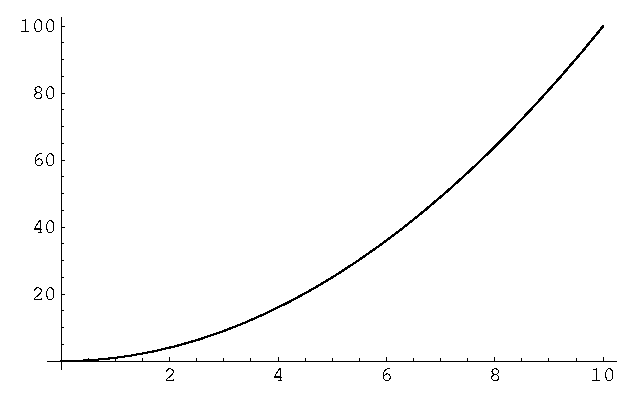
\includegraphics{plot.eps}
  \caption{%
    By default figures are not centered.
    This is a long caption to demonstrate that captions are single spaced.
  }
  \label{fi:not-centered}
\end{figure}

\Repeat{This is the second paragraph.}{10}

\begin{figure}[h]
  \centering
  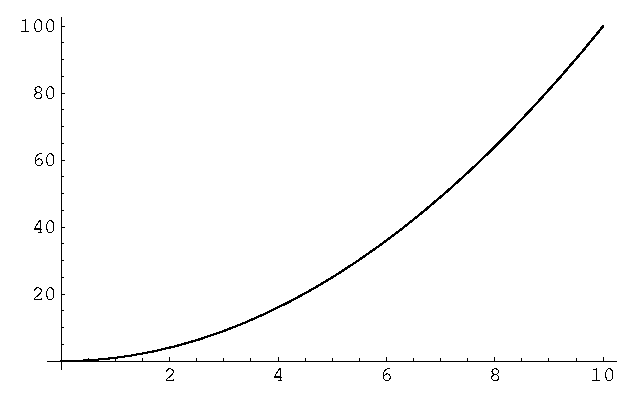
\includegraphics{plot.eps}
  \caption{Use {\tt \char'134centering\/} to center figures.}
  \label{fi:centered}
\end{figure}

\Repeat{This is the third paragraph.}{15}

\begin{figure}[h]
  \centering
  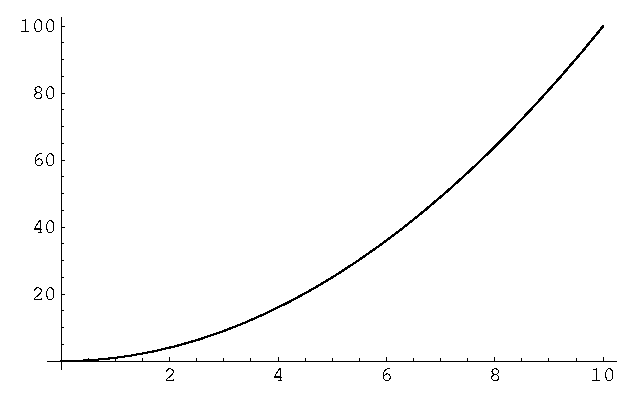
\includegraphics{plot.eps}
  \caption{This is another figuure.}
  \label{fi:another}
\end{figure}

\Repeat{This is the fourth paragraph.}{10}

\begin{figure}[h]
  \centering 
  \subfigure[First subcaption.]{\label{sf:two-parts-a}  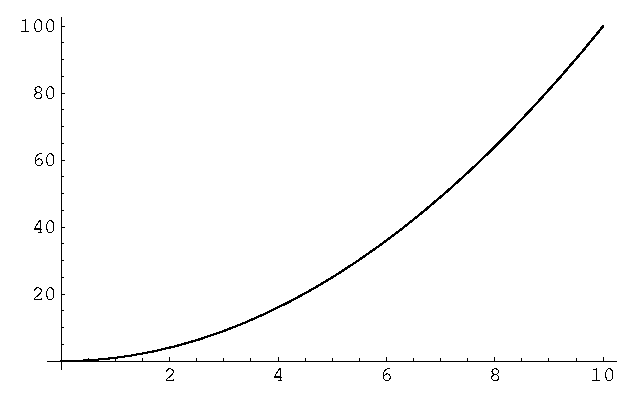
\includegraphics[width=0.3\textwidth]{plot.eps}}%
  \hskip 0.5truein
  \subfigure[Second subcaption.]{\label{sf:two-parts-b}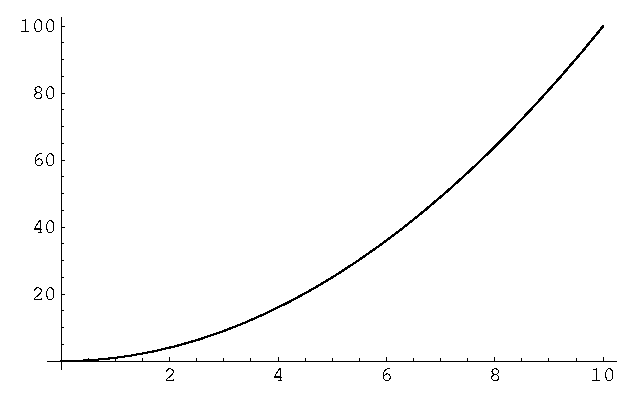
\includegraphics[width=0.3\textwidth]{plot.eps}}
  \caption{This figure has two parts.}
  \label{fi:two-parts}
\end{figure}

\Repeat{This is the fifth paragraph.}{10}

\begin{figure}[h]
  \centering
  \subfigure[First subcaption.]{\label{sf:four-parts-a}  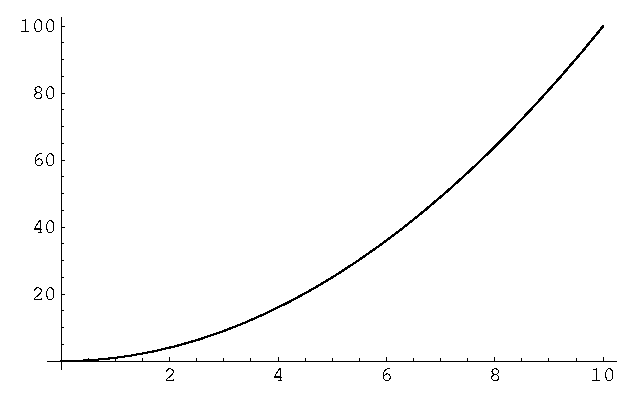
\includegraphics[width=0.3\textwidth]{plot.eps}}%
  \hskip 0.5truein
  \subfigure[Second subcaption.]{\label{sf:four-parts-b}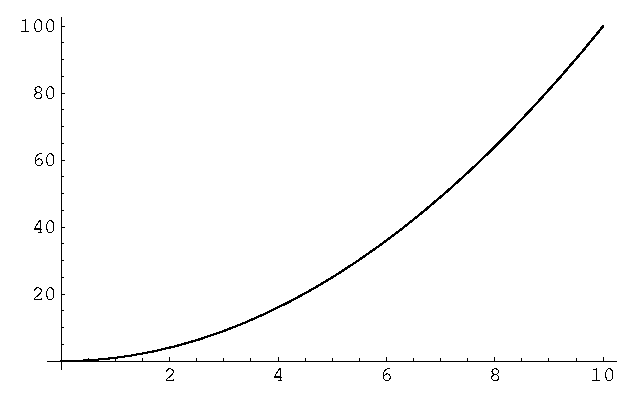
\includegraphics[width=0.3\textwidth]{plot.eps}}
  \subfigure[Third subcaption.]{\label{sf:four-parts-c}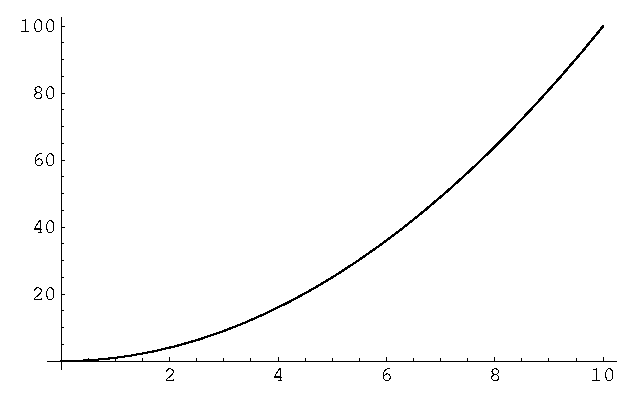
\includegraphics[width=0.3\textwidth]{plot.eps}}%
  \hskip 0.5truein
  \subfigure[Fourth subcaption.]{\label{sf:four-parts-d}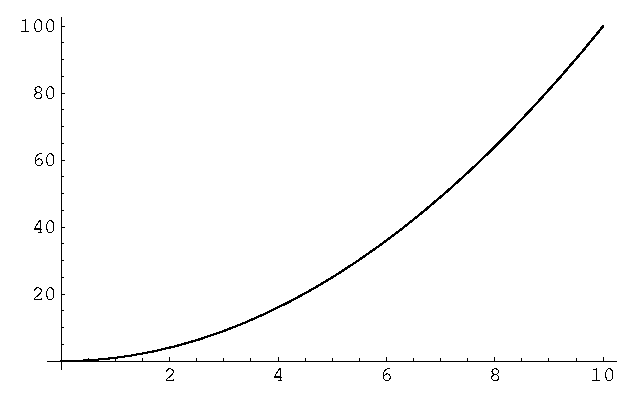
\includegraphics[width=0.3\textwidth]{plot.eps}}
  \caption{This figure has four parts.}
  \label{fi:four-parts}
\end{figure}

\Repeat{This is the sixth paragraph.}{10}

%%
%  THIS FILE DOES SOME UNUSUAL THINGS TO MAKE
%  IT EASIER TO DO DEMONSTRATIONS.  IT SHOULD
%  NOT BE USED AS AN EXAMPLE OF HOW TO PREPARE
%  A FILE.  SEE THE OUTPUT OF THIS FOR LATEX
%  INPUT AND OUTPUT EXAMPLES.
%




%
%  demo-mathematics.tex  2008-12-09  Mark Senn  http://engineering.purdue.edu/~mark
%

\chapter{Demonstrate Mathematics}

    % Use single spacing.
    \Baselinestretch{1}

    % You don't normally need this.
    \mbox{}

    \begin{verbatim}
% From _More Math Into LaTeX_, 4th Edition, page 152:
%     TeX uses $$ to open and close a displayed math environment.
%     In LaTeX, this may occassionally cause problems.  Don't do it.
\[
    E = mc^2
\]
    \end{verbatim}
% From _More Math Into LaTeX_, 4th Edition, page 152:
%     TeX uses $$ to open and close a displayed math environment.
%     In LaTeX, this may occassionally cause problems.  Don't do it.
\[
    E = mc^2
\]
    \vskip\baselineskip
    \hrule
    \vskip0.5\baselineskip
    \filbreak

    \begin{verbatim}
\begin{equation}
    E = mc^2
\end{equation}
    \end{verbatim}
\begin{equation}
    E = mc^2
\end{equation}
    \vskip\baselineskip
    \hrule
    \vskip0.5\baselineskip
    \filbreak

    \begin{verbatim}
% Mydefs.tex defines \be to be \begin{equation} and
% \ee to be \end{equation}.
\be
    E = mc^2
\ee
    \end{verbatim}
% Mydefs.tex defines \be to be \begin{equation} and
% \ee to be \end{equation}.
\be
    E = mc^2
\ee
    \vskip\baselineskip
    \hrule
    \vskip0.5\baselineskip
    \filbreak

    \begin{verbatim}
\be
    x = -\frac{b}{2a} \pm \frac{\sqrt{b^2 - 4ac}}{2a}
\ee
    \end{verbatim}
\be
    x = -\frac{b}{2a} \pm \frac{\sqrt{b^2 - 4ac}}{2a}
\ee
    \vskip\baselineskip
    \hrule
    \vskip0.5\baselineskip
    \filbreak

    \begin{verbatim}
% requires \usepackage{amsmath}; use align* for no equation number
\begin{align}
    a = {}& b + c\\
    x = {}& y + z
\end{align}
    \end{verbatim}
% requires \usepackage{amsmath}; use align* for no equation number
\begin{align}
    a = {}& b + c\\
    x = {}& y + z
\end{align}
    \vskip\baselineskip
    \hrule
    \vskip0.5\baselineskip
    \filbreak

    \begin{verbatim}
\[
    Z = \left(
        \begin{array}{cc}
            a& b\\
            c& d
        \end{array}
    \right)
\]
    \end{verbatim}
\[
    Z = \left(
        \begin{array}{cc}
            a& b\\
            c& d
        \end{array}
    \right)
\]
    \vskip\baselineskip
    \hrule
    \vskip0.5\baselineskip
    \filbreak

    \begin{verbatim}
\begin{equation}
    \begin{split}
        a = {}& b + c\\
            {}& + d + e
    \end{split}      
\end{equation}
    \end{verbatim}
\begin{equation}
    \begin{split}
        a = {}& b + c\\
            {}& + d + e
    \end{split}      
\end{equation}
    \vskip\baselineskip
    \hrule
    \vskip0.5\baselineskip
    \filbreak

    \begin{verbatim}
\be
    (\cos x)^2 + (\sin x)^2 = 1
\ee
    \end{verbatim}
\be
    (\cos x)^2 + (\sin x)^2 = 1
\ee
    \vskip\baselineskip
    \hrule
    \vskip0.5\baselineskip
    \filbreak

    \begin{verbatim}
If $X = \cos x$ and $Y = \sin x$ then $X^2 + Y^2 = 1$.
    \end{verbatim}
If $X = \cos x$ and $Y = \sin x$ then $X^2 + Y^2 = 1$.
    \vskip\baselineskip
    \hrule
    \vskip0.5\baselineskip
    \filbreak

%%
%  demo-multicols.tex  2007-03-19  Mark Senn  http://www.ecn.purdue.edu/~mark
%
%  Demonstrate multicols.
%
%  The multicols package must be loaded for this to work.
%  To load the multicols package put
%      \usepackage{multicols}
%  between the "\documentclass" and "\begin{document}" commands.
%

\chapter{Demonstrate Multicols}

% Put this amount of space between the columns.
\setlength{\columnsep}{0.5truein}

% Separate the columns with a vertical rule this wide.
\setlength{\columnseprule}{0.4pt}

\Repeat{This is one column.}{25}

\begin{multicols}{2}
\Repeat{This is two columns.}{25}
\end{multicols}

\begin{multicols}{3}
\Repeat{This is three columns.}{25}
\end{multicols}

\begin{multicols}{4}
\Repeat{This is four columns.}{25}
\end{multicols}

\begin{multicols}{5}
\Repeat{This is five columns.}{25}
\end{multicols}

%%
%  demo-tables.tex  2013-03-29  Mark Senn  http://engineering.purdue.edu/~mark
%
%  Demonstrate how to do tables.
%

\chapter{Demonstrate Tables}

% \newlength{\ta}
% \newlength{\tb}
% \newlength{\tc}
% 
% \settowidth{\ta}{\vbox{\hbox{Money}\hbox{Market}}}
% \settowidth{\tb}{\vbox{\hbox{Stocks}\hbox{and}\hbox{Bonds}}}
% \settowidth{\tc}{\vbox{\hbox{Money}\hbox{Market}\hbox{and}\hbox{Stocks}}}
% 
% {
%     \renewcommand{\baselinestretch}{1}
%     \begin{table}
%       \caption{%
%         \hfil Allocation of the IRA and Keogh Wealth\hfil\break
%         \mbox{}\hfil for Investors With or Without Brokerage Accounts\hfil
%       }
%       \label{tab:ira}
%       \begin{center}
%         \begin{tabular}%
%           {%
%             |%
%             c%
%             |%
%             >{\centering\hspace{0pt}}m{\the\ta}%  Money Market
%             |%
%             c%                                    Stocks 
%             |%
%             c%                                    Bonds
%             |%
%             c%                                    Diversified
%             |%
%             >{\centering\hspace{0pt}}m{\the\tb}%  Stocks and Bonds
%             |%
%             >{\centering\hspace{0pt}}m{\the\tc}%  Money Market and Stocks
%             |%
%             c%                                    Others
%             |%
%           }
%           \hline
%           IMP&
%             Money Market&
%             Stocks&
%             Bonds&
%             Diversified&
%             Stocks and Bonds&
%             Money Market and Stocks&
%             Others\tabularnewline
%           \hline
%           1& 14.19\%& 57.71\%& 12.21\%& 4.50\%& 7.36\%& 3.04\%& 0.99\%\tabularnewline \hline
%           2& 14.08\%& 58.18\%& 12.32\%& 4.44\%& 7.30\%& 2.80\%& 0.88\%\tabularnewline \hline
%           3 &14.26\%& 58.09\%& 12.27\%& 4.50\%& 7.19\%& 2.75\%& 0.94\%\tabularnewline \hline
%           4 &13.94\%& 58.11\%& 12.14\%& 4.78\%& 7.35\%& 2.68\%& 0.99\%\tabularnewline \hline
%           5 &13.92\%& 58.13\%& 11.93\%& 4.56\%& 7.60\%& 2.98\%& 0.88\%\tabularnewline \hline
%         \end{tabular}
%       \end{center}
%       This table presents the allocations of the wealth in the IRA
%       and Keogh accounts in various asset classes.
%       Results from each set of imputed data are presented here.
%       The first column lists the number of the imputations,
%       and rest of the columns lists various allocations.
%       Entrees under each asset class show the percentage of investors
%       who have most of their IRA
%       and Keogh wealth invested in that particular asset class.
%       The asset class Diversified
%       includes stocks,
%       bonds,
%       and money market investments.
%       The asset class Others
%       include investments in various life insurance products,
%       annuities,
%       real estate, etc.
%       \medskip
%     \footnotesize SOURCE: Survey of Consumer Finances,
%     2001,
%     Federal Reserve Board,
%     USA.\par
%   \end{table}
% }

Here is a really simple table.

% "h" means put table here---don't let it float to top or bottom of page
\begin{table}[h]
  \caption{American Presidents}
  \begin{center}
    \begin{tabular}{rl}
      \bf Number& \bf Name\\
      1& George Washington\\
      2& John Adams\\
      3& Thomas Jefferson\\
    \end{tabular}
  \end{center}
  \label{ta:American-Presidents}
\end{table}

There are 72.27 points per inch.
I like to put 2 points of vertical space between the heading
(Number Name)
and the first line
(1 George Washington)
of the table.

\begin{table}[h]
  \caption{American Presidents with 2pt vertical space after heading}
  \begin{center}
    \begin{tabular}{rl}
      \bf Number& \bf Name\\[2pt]  % put 2pt vertical space after this line
      1& George Washington\\
      2& John Adams\\
      3& Thomas Jefferson\\
    \end{tabular}
  \end{center}
  \label{ta:American-Presidents-with}
\end{table}

\LaTeX\ can print horizontal and vertical rules in tables.
I don't like the way this looks.

\begin{table}[h]
  \caption{American Presidents with horizontal and vertical lines}
  \begin{center}
    % "|" prints a vertical rule, "c" means center
    \begin{tabular}{|c|l|}
      % "\hline" prints a horizontal rule
      \hline
      \bf\#& \bf Name\\
      \hline
      1& George Washington\\
      \hline
      2& John Adams\\
      \hline
      3& Thomas Jefferson\\
      \hline
    \end{tabular}
  \end{center}
  \label{ta:American-Presidents-with}
\end{table}

\newpage

Here is a more complicated table.

\begin{table}[h]
  \caption{C Bitwise Operators}
  \begin{center}
    % "|" prints a vertical rule, "c" means center
    \begin{tabular}{cccc}
      \bf A& \bf B& \bf A$|$B& \bf A\&B\\[2pt]
      0& 0& 0& 0\\
      0& 1& 1& 0\\
      1& 0& 1& 0\\
      1& 1& 1& 1\\
    \end{tabular}
  \end{center}
  \label{ta:C-Bitwise}
\end{table}

You can use Plain \TeX's \verb+\halign+ command to make tables also.
If you can't do a complicated table using \LaTeX\ commands
you may want to try using Plain \TeX\ commands.
\LaTeX's table making commands use Plain \TeX\ commands.

\begin{table}[h]
  \caption{American Presidents using {\tt\char'134 halign}}
  \hbox to \textwidth{\hss\vbox{\halign{%
    \strut #&      % 0. \strut
    \hfil#\qquad&  % 1. Number
    #\hfil\cr      % 2. Name
    %
    & \bf Number& \bf Name\cr
    \noalign{\vskip 2pt}
    & 1& George Washington\cr
    & 2& John Adams\cr
    & 3& Thomas Jefferson\cr
  }}\hss}
  \label{ta:American-Presidents-using}
\end{table}

The next page shows how to do a table that is too long to fit on one page.

\newpage

% This is loosely based on page 106 of _A Guide to LaTeX_, third edition,
% by Helmut Kopka and Patrick W. Daly.
\begin{longtable}{|l|l|}
    \caption{State Abbreviations}\\
    \hline
    State& Abbreviation\\
    \hline
  \endfirsthead
    \caption[]{\emph{continued}}\\
    \hline
    State& Abbreviation\\
    \hline
  \endhead
    \hline
    \multicolumn{2}{r}{\emph{continued on next page}}
  \endfoot
    \hline
  \endlastfoot
  Alabama& AL\\
  Alaska& AK\\
% American Samoa& AS\\
  Arizona& AZ\\
  Arkansas& AR\\
% Armed Forces Europe& AE\\
% Armed Forces Pacific& AP\\
% Armed Forces the Americas& AA\\
  California& CA\\
  Colorado& CO\\
  Connecticut& CT\\
  Delaware& DE\\
% District of Columbia& DC\\
% Federated States of Micronesia& FM\\
  Florida& FL\\
  Georgia& GA\\
% Guam& GU\\
  Hawaii& HI\\
  Idaho& ID\\
  Illinois& IL\\
  Indiana& IN\\
  Iowa& IA\\
  Kansas& KS\\
  Kentucky& KY\\
  Louisiana& LA\\
  Maine& ME\\
% Marshall Islands& MH\\
  Maryland& MD\\
  Massachusetts& MA\\
  Michigan& MI\\
  Minnesota& MN\\
  Mississippi& MS\\
  Missouri& MO\\
  Montana& MT\\
  Nebraska& NE\\
  Nevada& NV\\
  New Hampshire& NH\\
  New Jersey& NJ\\
  New Mexico& NM\\
  New York& NY\\
  North Carolina& NC\\
  North Dakota& ND\\
% Northern Mariana Islands& MP\\
  Ohio& OH\\
  Oklahoma& OK\\
  Oregon& OR\\
  Pennsylvania& PA\\
% Puerto Rico& PR\\
  Rhode Island& RI\\
  South Carolina& SC\\
  South Dakota& SD\\
  Tennessee& TN\\
  Texas& TX\\
  Utah& UT\\
  Vermont& VT\\
% Virgin Islands& VI\\
  Virginia& VA\\
  Washington& WA\\
  West Virginia& WV\\
  Wisconsin& WI\\
  Wyoming& WY\\
\end{longtable}

\newcommand{\cbackslash}{\char'134}
\newcommand{\copencurly}{\char'173}
\newcommand{\cclosecurly}{\char'175}

\newlength{\twidth}
\newlength{\theight}

\setlength{\twidth}{\textwidth}
\setlength{\theight}{\textheight}

\begin{sidewaystable}
  % The following two lines compensate for what I think is a bug.
  \setlength{\textwidth}{\theight}
  \setlength{\textheight}{\twidth}
  \caption{%
    sidewaystable
    {\tt\cbackslash begin\copencurly tabular\cclosecurly\/}%
    \ldots
    {\tt\cbackslash end\copencurly tabular\cclosecurly\/}%
  }
  \begin{center}
    \begin{tabular}{rl}
      \bf Number& \bf Name\\[2pt]  % put 2pt vertical space after this line
      1& George Washington\\
      2& John Adams\\
      3& Thomas Jefferson\\
    \end{tabular}
  \end{center}
\end{sidewaystable}

\begin{sidewaystable}
  % The following two lines compensate for what I think is a bug.
  \setlength{\textwidth}{\theight}
  \setlength{\textheight}{\twidth}
  \caption{%
    sidewaystable
    {\tt\cbackslash halign\copencurly}\ldots{\tt\cclosecurly\/} table%
  }
  \hbox to \textwidth{\hss\vbox{\halign{%
    \strut #&      % 0. \strut
    \hfil#\qquad&  % 1. Number
    #\hfil\cr      % 2. Name
    %
    & \bf Number& \bf Name\cr
    \noalign{\vskip 2pt}
    & 1& George Washington\cr
    & 2& John Adams\cr
    & 3& Thomas Jefferson\cr
  }}\hss}
\end{sidewaystable}

%\newlength{\ta}
%\settowidth{\ta}{\vbox{\hbox{Money}\hbox{Market}}}
%\newlength{\tb}
%\settowidth{\tb}{\vbox{\hbox{Stocks}\hbox{and}\hbox{Bonds}}}
%\newlength{\tc}
%\settowidth{\tc}{\vbox{\hbox{Money}\hbox{Market}\hbox{and}\hbox{Stocks}}}
%
%  {\renewcommand{\baselinestretch}{1}
%\begin{table}
%  \caption{\hfil Allocation of the IRA and Keogh Wealth\hfil\break\mbox{}\hfil for Investors With or Without Brokerage Accounts\hfil}
%  \label{tab:ira}
%  \begin{center}
%    \begin{tabular}%
%      {%
%        |%
%        c%
%        |%
%        >{\centering\hspace{0pt}}m{\the\ta}%  Money Market
%        |%
%        c%                                    Stocks 
%        |%
%        c%                                    Bonds
%        |%
%        c%                                    Diversified
%        |%
%        >{\centering\hspace{0pt}}m{\the\tb}%  Stocks and Bonds
%        |%
%        >{\centering\hspace{0pt}}m{\the\tc}%  Money Market and Stocks
%        |%
%        c%                                    Others
%        |%
%      }
%      \hline
%      IMP&
%        Money Market&
%        Stocks&
%        Bonds&
%        Diversified&
%        Stocks and Bonds&
%        Money Market and Stocks&
%        Others\tabularnewline
%      \hline
%      1& 14.19\%& 57.71\%& 12.21\%& 4.50\%& 7.36\%& 3.04\%& 0.99\%\tabularnewline \hline
%      2& 14.08\%& 58.18\%& 12.32\%& 4.44\%& 7.30\%& 2.80\%& 0.88\%\tabularnewline \hline
%      3 &14.26\%& 58.09\%& 12.27\%& 4.50\%& 7.19\%& 2.75\%& 0.94\%\tabularnewline \hline
%      4 &13.94\%& 58.11\%& 12.14\%& 4.78\%& 7.35\%& 2.68\%& 0.99\%\tabularnewline \hline
%      5 &13.92\%& 58.13\%& 11.93\%& 4.56\%& 7.60\%& 2.98\%& 0.88\%\tabularnewline \hline
%    \end{tabular}
%  \end{center}
%  This table presents the allocations of the wealth in the IRA
%  and Keogh accounts in various asset classes.
%  Results from each set of imputed data are presented here.
%  The first column lists the number of the imputations,
%  and rest of the columns lists various allocations.
%  Entrees under each asset class show the percentage of investors
%  who have most of their IRA
%  and Keogh wealth invested in that particular asset class.
%  The asset class Diversified
%  includes stocks,
%  bonds,
%  and money market investments.
%  The asset class Others
%  include investments in various life insurance products,
%  annuities,
%  real estate, etc.
%  \medskip
%  \footnotesize SOURCE: Survey of Consumer Finances,
%  2001,
%  Federal Reserve Board,
%  USA.\par
%\end{table}
%  }


%%
%  demo-text.tex  2007-07-17  Mark Senn  http://engineering.purdue.edu/~mark
%

\chapter{Demonstrate Text}

% Use single spacing.
\Baselinestretch{1}

% You don't normally need this.
\mbox{}


%\vbox{
\begin{verbatim}
This is a sentence.
This is a sentence.
This is a sentence.
This is a sentence.
This is a sentence.

This is a sentence.
This is a sentence.
This is a sentence.
This is a sentence.
This is a sentence.
\end{verbatim}
This is a sentence.
This is a sentence.
This is a sentence.
This is a sentence.
This is a sentence.

This is a sentence.
This is a sentence.
This is a sentence.
This is a sentence.
This is a sentence.
\vskip\baselineskip
\hrule
%}
\vskip0.5\baselineskip
\filbreak

%\vbox{
\begin{verbatim}
From \verb+http://www.biblegateway.com/passage/?book_id=1&chapter=1&version=50+:

\begin{quote}
    1 In the beginning God created the heavens and the earth.
    2 The earth was without form,
    and void;
    and darkness was on the face of the deep.
    And the Spirit of God was hovering over the face of the waters.

    3 Then God said,``Let there be light'';
    and there was light.
    4 And God saw the light,
    that it was good;
    and God divided the light from the darkness.
    5 God called the light Day,
    and the darkness He called Night.
    So the evening and the morning were the first day. 
\end{quote}
\end{verbatim}
From \verb+http://www.biblegateway.com/passage/?book_id=1&chapter=1&version=50+:

\begin{quote}
    1 In the beginning God created the heavens and the earth.
    2 The earth was without form,
    and void;
    and darkness was on the face of the deep.
    And the Spirit of God was hovering over the face of the waters.

    3 Then God said,``Let there be light'';
    and there was light.
    4 And God saw the light,
    that it was good;
    and God divided the light from the darkness.
    5 God called the light Day,
    and the darkness He called Night.
    So the evening and the morning were the first day. 
\end{quote}
\vskip\baselineskip
\hrule
%}
\vskip0.5\baselineskip
\filbreak

%\vbox{
\begin{verbatim}
\begin{description}
    \item[apple]
        A red fruit.
    \item[banana]
        A yellow fruit.
        This sentence is to make the entry longer so you can see what happens.
        This sentence is to make the entry longer so you can see what happens.
    \item[cherry]
        A red friut.
\end{description}
\end{verbatim}
\begin{description}
    \item[apple]
        A red fruit.
    \item[banana]
        A yellow fruit.
        This sentence is to make the entry longer so you can see what happens.
        This sentence is to make the entry longer so you can see what happens.
    \item[cherry]
        A red friut.
\end{description}
\vskip\baselineskip
\hrule
%}
\vskip0.5\baselineskip
\filbreak

%\vbox{
\begin{verbatim}
\begin{enumerate}
    \item apple
    \item banana
        This sentence is to make the entry longer so you can see what happens.
        This sentence is to make the entry longer so you can see what happens.
    \item cherry
\end{enumerate}
\end{verbatim}
\begin{enumerate}
    \item apple
    \item banana
        This sentence is to make the entry longer so you can see what happens.
        This sentence is to make the entry longer so you can see what happens.
    \item cherry
\end{enumerate}
\vskip\baselineskip
\hrule
%}
\vskip0.5\baselineskip
\filbreak


%\vbox{
\begin{verbatim}
\begin{itemize}
    \item apple
    \item banana
        This sentence is to make the entry longer so you can see what happens.
        This sentence is to make the entry longer so you can see what happens.
    \item cherry
\end{itemize}
\end{verbatim}
\begin{itemize}
    \item apple
    \item banana
        This sentence is to make the entry longer so you can see what happens.
        This sentence is to make the entry longer so you can see what happens.
    \item cherry
\end{itemize}
\vskip\baselineskip
\hrule
%}
\vskip0.5\baselineskip
\filbreak


% Notes and footnotes are optional.
% Reference: TM 34.
% I have not implemented this yet.  Mark Senn 2002-06-03
%%\chapter{Notes}

\begin{itemize}
	\item Do we hash node's id in the commitment field of its data-item? NO
	\item Do we send the payload signature in case of Figure 5.4? YES
\end{itemize}

To do list:
\begin{itemize}
	% \item ch-3: signatures from 628; All PKI are not digital signatures capable.
	% \item ch-5: Clear goals of the protocol.
	% \item Review the writing.
	% \item ch-2: Add smooth transition to the security section.
	% \item ch-2: add more applications in section 2.1.
	% \item ch-4: change sign label
	% \item ch-4: Why SHIA does not have ID in their label? Why do you have ID? What benefits you get out of it?
	\item Cheating: Finish writing about detecting a cheater.
	\item ch-4: Image modifications. Update images with darker borders. Decrease width. Save word as pdf and then crop images
	\item Review the writing.

	\item 3. Discuss cheating, distributing off-path.  
	\item ch-6: Why don't you need signatures with off-path?
	\item ch-4: Advantages of signing the B's payload.

	\item ch-3: cite book for digital signatures

	\item ch-6: removing old signatures, and signing those again
	\item ch-6: equation for number of certificates needed in the network

\end{itemize}

% A vita is optional for masters theses
% and required for doctoral dissertations.
% Reference: TM 13.
% CHANGE NEXT LINE?
%%
%  vita.tex   2003.07.23  14:59:33   Mark Senn <mds@purdue.edu>
%
%  This is the vita for a simple, example thesis.
%
%  A vita is required only in a doctoral dissertation.
%

\begin{vita}
    [Put a brief autobiographical sketch here.]
\end{vita}


\end{document}

% LaTeX won't read after the \end{document} command.
% You can put notes to yourself or LaTeX input not
% ready for use here if you'd like.
